% !TeX root = ../main-presentation.tex
\begin{frame}
    \frametitle{What are we going to be talking about?}
    \pause
    \centering
    \LARGE
    Digital circuits!

    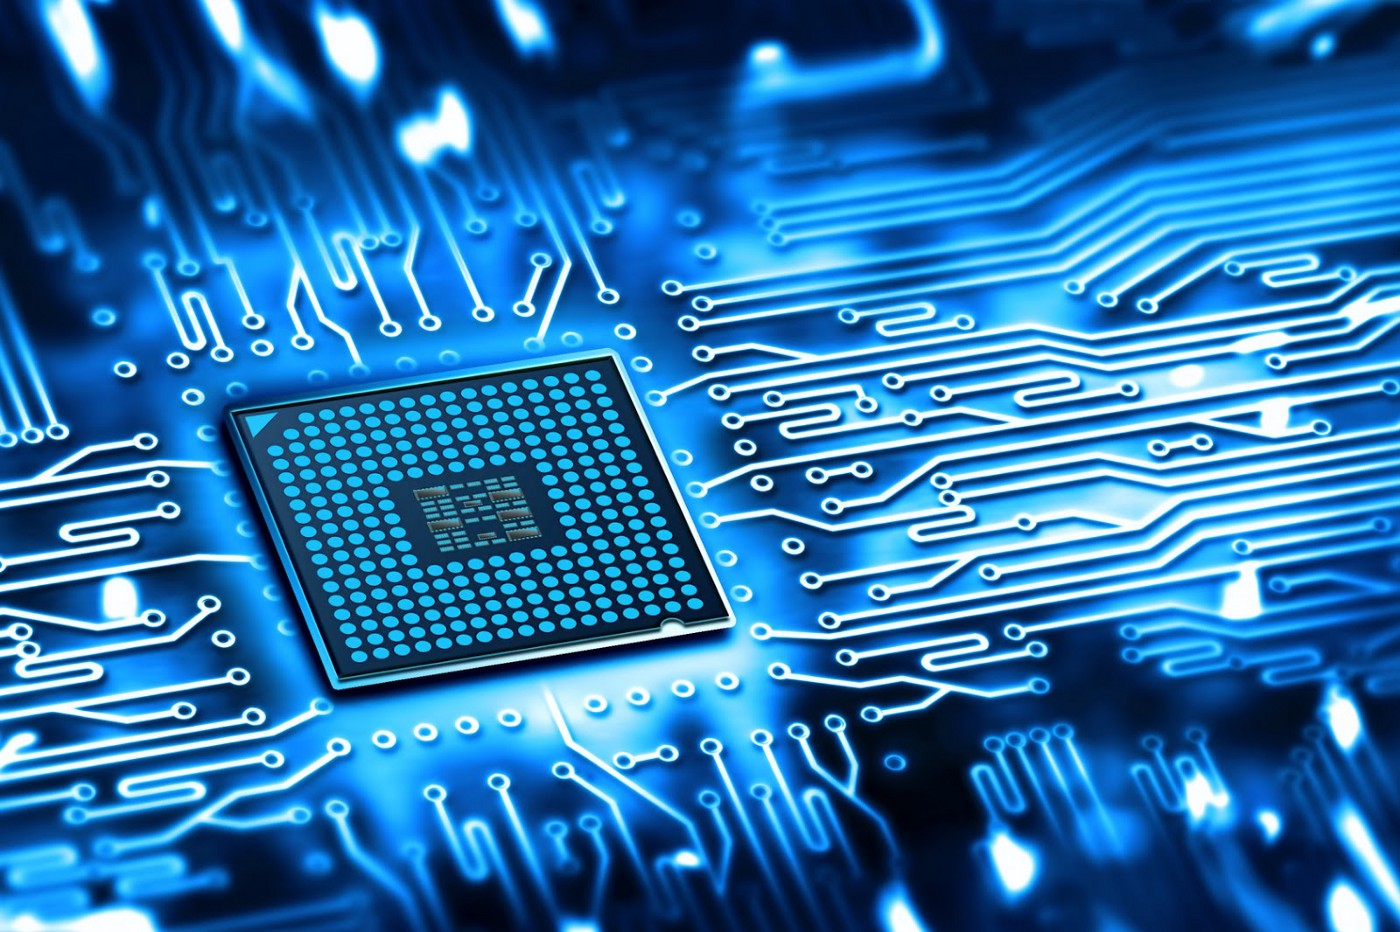
\includegraphics[width=0.6\textwidth]{imgs/circuit}
\end{frame}
\begin{frame}
    \frametitle{What are we going to be talking about?}
    \centering
    \LARGE
    Digital circuits!

    \vspace{1em}
    \normalsize

    \scalebox{2}{\tikzfig{circuits/examples/sr-latch/real-circuit}}
\end{frame}
\begin{frame}
    \frametitle{What are we going to be talking about?}

    \pause

    \centering
    \LARGE
    We want a \alert{compositional} theory of digital circuits.

    \vspace{0.5em}

    \normalsize

    \pause
    \dsptikzfig{strings/category/f}[box=F,colour=seq]
    \pause
    \quad
    \dsptikzfig{strings/category/f}[box=G,colour=seq]
    \pause
    \quad
    \dsptikzfig{strings/category/f-2-2}[box=H,colour=seq]

    \pause
    \vspace{1em}

    \dsptikzfig{strings/category/seq}[box1=F,box2=G,colour=seq]
    \quad
    \dsptikzfig{strings/monoidal/tensor}[box1=F,box2=G,colour=seq]
    \quad
    \dsptikzfig{strings/traced/trace-rhs}[box=H,colour=seq]

\end{frame}

\begin{frame}
    \frametitle{Why all the pictures?}
    \centering

    \LARGE
    We want to reason \alert{equationally} about circuits.

    \pause

    Using \alert{string diagrams} removes much of the bureacracy

\end{frame}
\begin{frame}
    \frametitle{What came before}

    \pause
    \alert{Lafont (2003)}
    \emph{`Towards an algebraic theory of Boolean circuits'}

    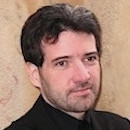
\includegraphics[width=0.15\textwidth]{imgs/lafont}

    \vspace{0.5em}
    \pause

    \alert{Ghica, Jung, Lopez (2017)}
    \emph{`Diagrammatic semantics for digital circuits'}

    \includegraphics[width=0.15\textwidth]{imgs/ghica}
    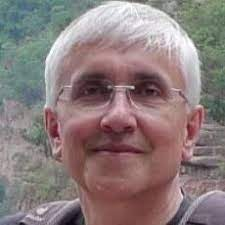
\includegraphics[width=0.15\textwidth]{imgs/achim}
    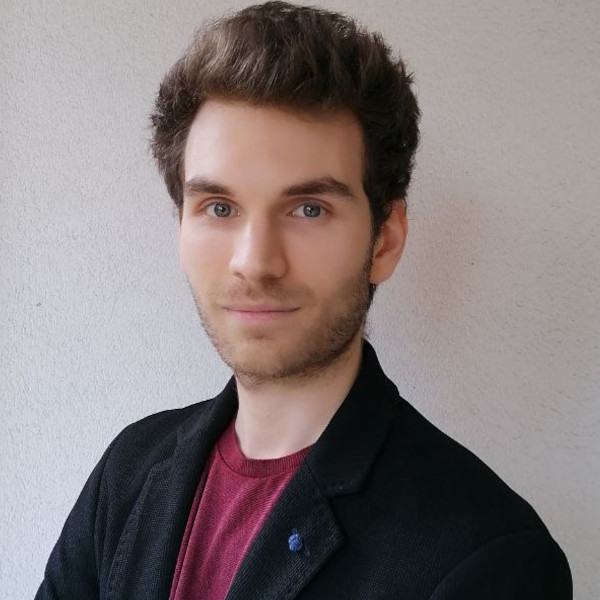
\includegraphics[width=0.15\textwidth]{imgs/lopez}
\end{frame}

\begin{frame}
    \frametitle{Joint work with...}
    \centering
    \begin{minipage}{0.4\textwidth}
        \centering

        \includegraphics[width=0.75\textwidth]{ghica}

        \vspace{0.5em}

        \alert{Dan Ghica}

        University of Birmingham
    \end{minipage}
    \qquad
    \begin{minipage}{0.4\textwidth}
        \centering
        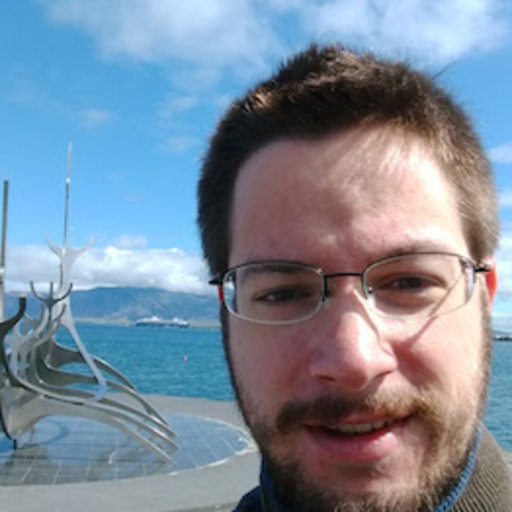
\includegraphics[width=0.75\textwidth]{sprunger}

        \vspace{0.5em}

        \alert{David Sprunger}

        Indiana State University
    \end{minipage}
\end{frame}